
\section{Relação Tempo-Frequência}
    
    \subsection{Contexto}
        Para o caso real, os sinais de áudio convoluem com a resposta ao impulso de um filtro, que representa o percurso realizado pelos mesmos entre as fontes e os sensores. Isto caracteriza um caso de misturas convolutivas (conforme visto na seção [referência]). 
        
        Com o conhecimento de que podemos representar uma operação de convolução no domínio tempo da mesma forma do que uma multiplicação no domínio da frequência, uma forma de simplificar este problema seria aplicar a transformada de Fourier à estes sinais, resolver múltiplos casos de misturas instântaneas e aplicar a transformada inversa de Fourier para levar os sinais de volta ao domínio do tempo. Uma das vantagens desta abordagem reside na redução da complexidade computacional e qualquer algoritimo ICA que trabalhe com números complexos e misturas instantâneas está apto para ser usado.
        
        Entretanto, as ambiguidades de escalamento e permutação inerentes ao problema de BSS (Seção [~\href{cap1}]), se tornam elementos centrais no processo de separação e precisam ser resolvidas. Ao trabalhar no domínio da frequência, a ICA fornece componentes independentes em cada raia de frequência, mas as as componentes de cada fonte não forem devidamente agrupadas antes de serem levadas para o domínio do tempo novamente. Isto é crucial para obter uma solução aceitável.
        
        Também é relevante citar o problema da circularidade da DFT. No caso discreto, o produto no domínio da frequência corresponde à convolução circular no domínio do tempo. Isto restringe o caso em que os filtros no domínio do tempo sejam periódicos, o que não é condizente com a realidade. Para fazer com que a multiplicação no domínio da frequência seja equivalente à convolução linear no domínio do tempo, é necessário que a representação do sinal no domínio do tempo deve ter um número de raias de frequência maior ou igual ao tamanho do filtro somado ao trecho do sinal, além do sinal ter de ser reconstruído através da técnica de Overlap-Add [referência]. Este processo é conhecido como \textit{FFT Filtering} e é amplamente utilizada para realizar convolução rápida de um filtro com um sinal longo. Quando isto não é respeitado, o sinal provinente do tratamento na frequência, seguido da sua IDFT será uma versão distorcida do sinal equivalente à convolução no domínio do tempo.
    
    \subsection{Sumário}
        O processo de tratamento do problema de FDBSS está ilustrado na Figura ~\ref{fig:frequencymodel} e pode ser estruturado da seguinte forma:
        
        \begin{enumerate}
            \item Inicialmente, transforma-se os vetores de misturas $\mathpzc{x_j}(n)$, j = 1,$\dots$,M em suas representações no domínio da frequência $\mathpzc{x_j}(m,k)$ , k = 0, $\dots$, K-1 (sendo \texit{m} o índice do \textit{frame} e K o número de raias de frequência), através da \textit{STFT}
            
            \item Como uma etapa de pré-processamento, realiza-se um branqueamento nos sinais, obtendo-se os sinais branqueados no domínio da frequência  $\mathpzc{z_j}(m,k)$ e a matriz branqueadora $\mathcal{V}$($\mathpzc{k}$).
            
            \item A etapa de processamento, que consiste na separação propriamente dita, é realizada, gerando uma matriz separadora $\mathcal{W}$($\mathpzc{k}$) para cada raia de frequência \texit{k}, além do vetor com as saídas separadas $\mathbf{y}$($\mathpzc{m,k})$ = [$\mathpzc{y_1}$($\mathpzc{m,k})$, $\dots$, $\mathpzc{y_N}$($\mathpzc{m,k})$]$^T$, sendo que tanto este quanto aquela estão fora de ordem e de magnitude.
            
            \item Já como um pós-processamento, são resolvidas as questões de permutação e escalamento, através das matries $\mathcal{P}$($\mathpzc{k})$ e $\Lambda$($\mathpzc{k})$.
            
            \item Por fim, é necessário levar o vetor com as saídas separadas novamente para o domínio do tempo através da \textit{ISTFT}.
            
        \end{enumerate}

        \begin{figure}[h!]
            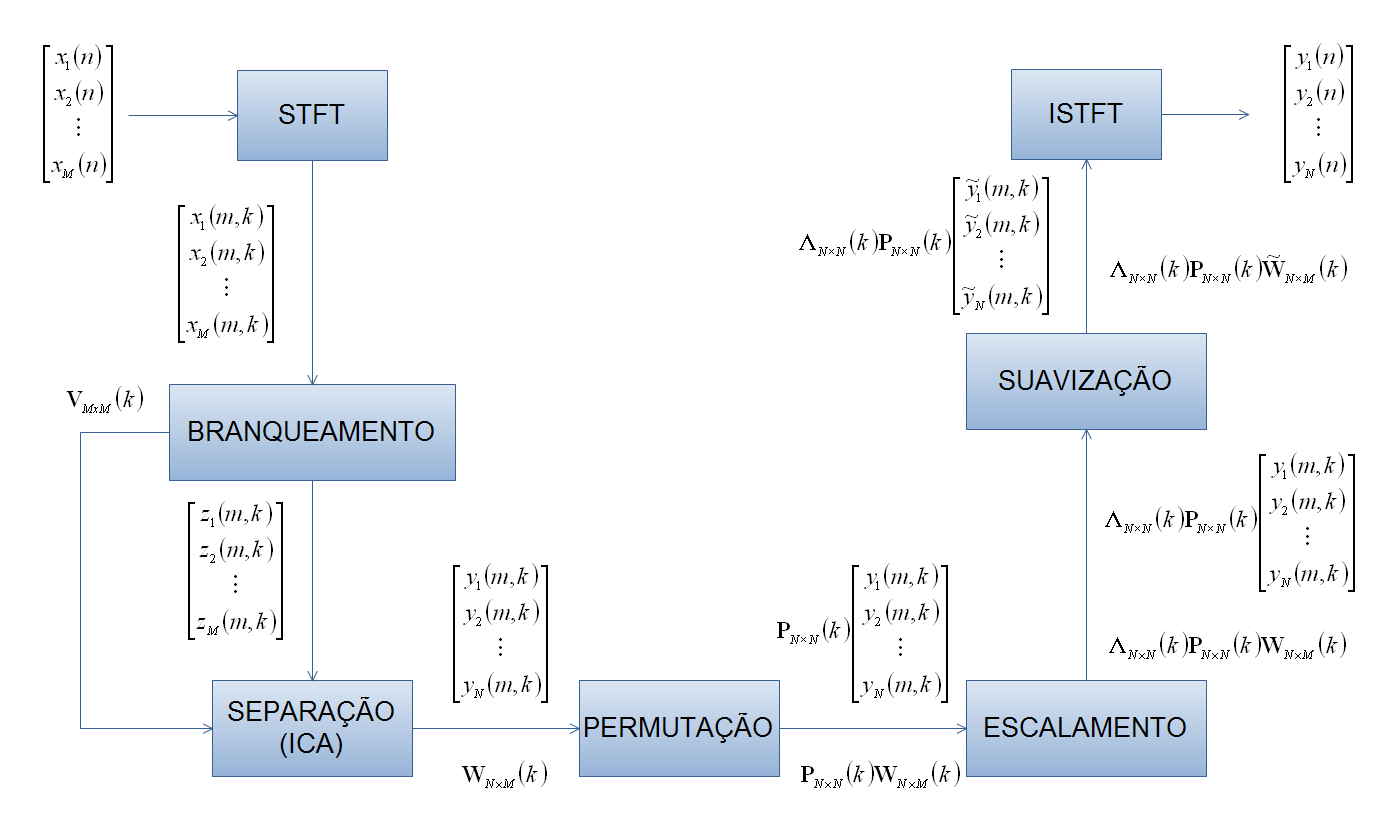
\includegraphics[scale=0.4]{frequencyprocess.png}
            \caption{Esquema do processo de FDBSS.}
            \label{fig:frequencymodel}
        \end{figure}

    \subsection{STFT}
        A STFT de um sinal x é dada pela equação abaixo (\ref{eq:STFT}), onde:

    %STFT
    \begin{equation}\label{eq:STFT}
        \mathcal{X}(\mathpzc{m},\mathpzc{k})
        = \sum_{n} \mathbf{x}(\mathpzc{n})
        \mathpzc{win}_\mathpzc{a}(\mathpzc{n} - \mathpzc{mJ})
        exp \left( -j \frac{2\pi\mathpzc{kn}}{K} \right), \mathpzc{k} = 0, \dots, K-1
    \end{equation}


        \begin{itemize}
            
            \item \mathpzc{k} é a raia de frequência, com intervalo [0, K-1]. Pode ser interpretada como a frequência discreta $\mathpzc{f_k}$ $\in$ \big\{0,$\frac{1}{K}$ $\mathpzc{f_s}$, \dots, $\frac{K-1}{K}$ $\mathpzc{f_s}$ \big\}.
                        
            \item K é o número de raias de frequência da DFT.
                        
            \item L é o comprimento da janela.
                        
            \item J é o deslocamento da janela.
            
            \item  $\mathpzc{f_s}$ é a frequência de amostragem.
            
            \item $\mathpzc{win_a}$($\mathpzc{n}$) é a janela de análise, definida como sendo não-nula apenas no intervalo [0, L-1]. O salto J é obviamente menor ou igual L, ou haverá perda de observações. Este saldo deve ser bem escolhido para não haver distorções na síntese dos sinais.
        \end{itemize}
    
        Pode-se notar que K=L na equação acima. Entretanto, há casos em que K$>$L, que são chamados de \textit{oversampled}. Nestes casos, é necessário fazer \textit{zero-padding} para preencher o sinal com zeros antes de passar para a frequência, conforme descrito em (\cite{STFT})
        
        A notação prática do cálculo da STFT está em (~\ref{eq:practiceSTFT}), onde:


        \begin{equation}\label{eq:practiceSTFT}
            \mathcal{X}(\mathpzc{m})
            = DFT(diag(\mathbf{x_{frame}}(\mathpzc{m})\mathbf{win_a}))
         \end{equation}
    
        \begin{enumerate}
        
            \item $\mathbf{DFT(v)}$ representa a DFT do vetor $\mathbf{v}$, que pode ser calculada através da FFT.
            
            \item O vetor $\mathbf{x_{frame}}$(m) = [$\mathpzc{x}$($\mathpzc{mJ}$), $\dots$, $\mathpzc{x(mJ + L - 1)}$]$^T$ tem comprimento L e representa o \textit{frame m} no domínio do tempo
            
            \item O vetor $\mathcal{X}(\mathpzc{m})$ = [$\mathcal{X}$($\mathpzc{f_0,m})$, $\dots$, $\mathcal{X}$($\mathpzc{f_{K-1},m}$)]$^T$ tem comprimento K e é o vetor com a representação em
            frequência do \texit{frame m}.
            
            \item O vetor $\mathbf{win_a}$ contém os elementos não nulos da janela mostrada em ~\ref{eq:STFT}. Assim sendo, tem comprimento L. O produto diag($\mathbf{x}$($\mathpzc{mJ}$))$\mathbf{win_a}$ resulta em um vetor de comprimento L. Por conta disos, se K $>$ L, devem ser realizado um \texit{zero-padding} de K - L amostras no final do vetor antes de aplicar a DFT.
        
        \end{enumerate}
        A notação prática do cálculo da ISTFT está em (~\ref{eq:practiceISTFT}) e (~\ref{eq:practiceISTFT2})
        
        \begin{equation}\label{eq:practiceISTFT}
            \mathbf{y_{frame}}(\mathpzc{m})
            = diag(\mathbf{win_s}IDFT(\mathcal{Y}(\mathpzc{m}))
         \end{equation}
        
        \begin{equation}\label{eq:practiceISTFT2}
            \mathbf{y}(\mathpzc{n})
            = \sum_{m}SHIFT(\mathbf{y_{frame}}(\mathpzc{m}),\mathpzc{mJ},\mathbf{N_{amost}})
         \end{equation}
        
        O sinal $\mathbf{y}$($\mathpzc{n}$) tem o comprimento de $N_{amost}$ e a operação SHIFT($\mathbf{a}$,b,c) desloca o vetor $\mathbf{a}$ de b amostras e aumenta seu comprimento para c, de forma que o vetor resultante tenha P elementos não-nulos, onde P é o tamanho do vetor $\mathbf{a}$.
        
        A técnica de \textit{Overlap-Add} consiste em acrescentar \textit{frames} superpostos para formar o sinal completo novamente. Também conhecida como OLA, esta técnica possui algumas variações, tais como a WOLA (\textit{Weighted Overlap-Add}) e a COLA (\textit{Constant Overlap-Add}). Esta técnica utiliza-se de uma janela de síntese $\mathpzc{win_s}(n)$ para a realização da ISTFT. Relacionar a janela de síntese $\mathpzc{win_s}(n)$ com a janela de análise $\mathpzc{win_a}(n)$ e os tamanhos dos comprimentos das janelas e dos sinais é fundamental para criar condições para que a transformação de volta para o domínio do tempo não possua distorções. 
        
        Para que a \textit{FFT Filtering} (necessária para resolver o problema de produto no domínio de  frequência discreta ser equivalente à convolução circular no domínio do tempo) gere um resultado satisfatório, as condições (\ref{eq:condition1}) e (\ref{eq:condition2}) devem ser satisfeitas. A condição (\ref{eq:condition2}) é chamada de condição COLA. Se não houver transformação ou a transformação for não-linear, a condição passa a ser (\ref{eq:condition3}). 
        
        \begin{equation}\label{eq:condition1}
            K \geq L + Q - 1
        \end{equation}
        
        \begin{equation}\label{eq:condition2}
            \sum_m \mathpzc{win_a(n - mJ) = c , c} constante, \forall\mathpzc{n} \in \mathbb{Z}
        \end{equation}
        
        \begin{equation}\label{eq:condition3}
            \sum_m \mathpzc{win_a(n - mJ)}\mathpzc{win_s(n - mJ) = c , c} constante, \forall\mathpzc{n} \in \mathbb{Z}
        \end{equation}
        
        
        Neste trabalho, iremos utilizar a janela de \texit{Hanning} (\ref{eq:hanning}) como janela de análise, atendendo à condição COLA (\ref{eq:condition2}). Para isto, usaremos J = $\frac{L}{2}$. Normalmente, a janela retangular é escolhida como a janela de síntese. Existem estudos acerca da utilização de outras janelas e em quais condições estas satisfazem ou não a COLA. Recomendamos a leitura de \cite{LuizVictorio} para maior aprofundamento no assunto.
        
        \begin{equation}\label{eq:hanning}
            \mathpzc{w_{hanning}(n)} = 0,5 \left( 1 - cos\frac{2\pi\mathpzc{n}}{L}\right)
        \end{equation}
        
\section{Pré-Processamento}
    O estágio de pré-processamento pode surgir de três formas: necessário, auxiliar ou desnecessário, dependendo do método de separação a ser empregado no processamento propriamente dito. O método mais comum de pré-processamento é o de \textit{branqueamento}, que se baseia na média do vetor de amostras.
    
    \subsection{Branqueamento}
        Em geral, branquear os vetores é uma boa prática, visto que faz grande parte do trabalho de separação, a descorrelação. Dependendo do método utilizado na etapa de separação, o branqueamento pode ser obrigatório (\textit{FastICA}) ou melhorar a velocidade e robustez da convergência do algoritmo ICA no domínio da frequência (\textit{Natural ICA}). A normalização do vetor de misturas desempenha um papel importante em sinais de áudio devido à sua característica de não-brancura (ou colorido), ou seja, a energia varia bastante entre as frequências.
        
        Matematicamente, é possivel mostrar que o processo de branqueamento faz aproximadamente metade do trabalho de separação, sem muito custo computacional. Entre outros benefícios, estão a rapidez e uniformidade na convergência para cada raia de frequência, quando utilizado um passo de adaptação fixo, além de ser pré-requistio dos algoritmos \textit{FastICA}.
        
        O processo é dividido em duas partes: A primeira consiste em fazer a centralização do vetor de misturas, isto é, fazer com que cada mistura possua média igual a zero. Feito isso, é necessário tornar a sua matriz de covariância igual à matriz identidade, resultando na descorrelação das componentes do vetor de amostras.
        
        A centralização pode ser realizada individualmente sobre cada uma das raias de frequência do vetor de amostras no domínio da frequência $\mathpzc{x_{jk}}(m)$, de forma a obter $\mathpzc{x_{jk}}(m)$ $\leftarrow$ $\mathpzc{x_{jk}}(m)$ - $\mathpzc{E}$$\{$$\mathpzc{x_{jk}(m)}$$\}$.
        
        Uma vez feita a centralização, tem-se que $\mathpzc{E}$$\{$$\mathbf{x}$$\}$ = 0 . Assim sendo, a matriz de covariância do vetor de misturas é dada por:
        
        \begin{equation}\label{eq:covariance}
            \sum_{\mathpzc{x_{k}x_{k}}} = \mathpzc{E}\{\mathbf{x_{k}x_{k}^H}\}
        \end{equation}
        
        O branqueamento se dá sobre cada frequência por uma matriz \mathbf{V}:
        
        \begin{equation}\label{eq:whiteningfrequency}
            \mathbf{z_k}(\mathpzc{m}) = \mathbf{V_k}\mathbf{x_k}(\mathpzc{m})
        \end{equation}
        
        para obtermos $\sum_{\mathpzc{z_{k}z_{k}}}$ = $\mathbf{I}$. Sabendo que $\sum_{\mathpzc{z_{k}z_{k}}}$= $\mathbf{V_k}$ $\sum_{\mathpzc{z_{k}z_{k}}}$ $\mathbf{V_k^H}$, ao decompormos $\sum_{\mathpzc{z_{k}z_{k}}}$ em razão das suas matrizes de autovalores e autovetores ($\sum_{\mathpzc{z_{k}z_{k}}}$ = $\mathbf{EDE^H}$), chegamos à conclusão de que:
        
        \begin{equation}\label{eq:vk}
            \mathbf{V_k} = \mathbf{D}^{-\frac{1}{2}}\mathbf{E^H}
        \end{equation}
        
        A matriz $\mathbf{E}$ é a matriz que contém os autoetores da matriz de correlação $\mathbf{R_{x_k}_{x_k}}$, onde cada coluna é um autovetor e e $\mathbf{D}$ é uma matriz diagonal que contém os autovalores de $\sum_{\mathpzc{x_{k}x_{k}}}$. O resultado interessante é que se perumtarmos as matrizes $\mathbf{D}$ e $\mathbf{E}$, o produto $\mathbf{D}^{-\frac{1}{2}}\mathbf{E^H}$ se mantém, contanto que a permutação aplicada seja igual nas duas matrizes.
        
        Este resultado diz que podemos manipular as matrizes $\mathbf{D}$ e $\mathbf{E}$ de forma que o autovetor corresponda ao seu autovalor. Isto implica diretamente na redução dimensional do problema, uma vez que as componentes princiais do vetor de misturas corresponderão às primeiras linhas do vetor branqueado. Esta redução dimensional é conhecido como Análise de Componentes Principais (PCA), do qual surgiu o conceito de ICA. 
\section{Processamento}
    \subsection{Separação}
\section{Pós-Processamento}
    \subsection{Escalonamento}
    \subsection{Permutação}